\documentclass{article}
\usepackage{graphicx} % Required for inserting images

\title{Requirements Analysis Report}
\author{Nikaela Balla
\and Mishkat Haider Chowdhury
\and Mauricio Guillermo Loza Arze}

\date{March 2023}

\begin{document}

\maketitle

\section{ Problem to be solved}
\label{sec:problem}
The purpose of this project is to make a SmartTable.Why would we need this? 
Well, imagine you are in a crowded restaurant. You have to wait for the host to bring you to a table that isn't reserved. Once you sit down,
you will need to grab the waiter's attention to order and then to get the bill. This is a lot of work for people with social anxiety or people 
who are disabled. That is the problem our table is implementing to fix. 
\section{ Introduction}
Our intended users are: a client in a restaurant and the waiter in the restaurant or other service-based establishments.
The client has difficulties communicating with others, because of social anxiety, disability, or other reasons. The waiter is overworked and
needs the help of the SmartTable to lessen his workload.
The different options for our interface implementation: \begin{itemize}
    \item Gesture-based interface using a leap motion sensor \cite{zaicti2015free}.
    \item  Voice control commands using a phone application.
    \item  Gestures-based interface using conventional cameras (OpenCV).
    \item A remote with buttons for changing the colors.
\end{itemize}

\subsection{Experience Sequence }
The customer enters the restaurant. The table has Led lights on its side that indicate the different states it has.
\begin{itemize}
    \item Table is green by default.
    \item  When the client sits on the table, its color changes to red. It uses simple pressure sensors to tell when someone is sitting \cite{cheng2013smart}.
    \item When the client wants to request the waiter's attention, they make a gesture, speak to the app, or press a button. 
    The table changes color from  red to blue.
    \item  There is  a timer that turns darker blue the more the client waits.
    \item Waiter approaches and turns off the timer in a similar way to the client, resets table status and it goes back to the color red.
    \item When the client requests the bill with a gesture, voice, or button, the table changes color to yellow.
    \item When the client sets the table to "do not disturb" in the same way as above, the table changes color to white.
    \item Waiter sets table to reserved status similarly as above, the table then changes to red.
\end{itemize}
This process will be explained in more detail in the requirements section.
\section{Requirements}
\subsection{Functional requirements}
\begin{itemize}
    \item The system should identify when a user is seated on the table.
    \item The system should provide an interface for both user types (client, waiter) to input commands.
    \item The system should visually show the confirmation of a command executed by both user types (client, waiter).
    \item The system should show visually the current state of the table.
    \item The system recognizes these commands: occupied table, the client wants to order, the client does not want to get disturbed, client requests the bill, table reserved.
    \item For each of the commands the visual confirmation should use a different color.
\end{itemize}
\subsection{Environmental requirements}
\begin{itemize}
    \item The system's visual indicators should be visible in a variety of lighting conditions.
    \item The system interface should be able to work under different light and sound conditions.
    \item The system's visual indicators should be visible no matter the position of the table.
    \item The system should not interfere with the intended use of the table.
    \item The system should withstand any incident common to restaurant tables.
\end{itemize}
\subsection{User characteristics}
\begin{itemize}
    \item Client: The expected skill set of the client is a novice.
    \item Waiter: The expected skill set of the waiter is expert.
\end{itemize}
\subsection{Usability goals}
\begin{itemize}
    \item The commands used by the client should be simple and easy to master.
    \item The commands used by the waiter should have a certain level of complexity, this should avoid replication from the client side. But at the same time be understandable and trainable by the workforce.
\end{itemize}
\subsection{User experience goals}
\begin{itemize}
    \item Using the command interface should be enjoyable to use.
    \item The system should be responsive when receiving commands.
\end{itemize}
\section{Requirement fulfillment}
The input of the system has three proposals ordered and with a focus on the first one:
\begin{itemize}
    \item Hand gestures with leap motion sensors.
    \item Voice commands via phone app.
    \item Hand gestures with a conventional video camera.
\end{itemize}
We have three proposals for the system but with a preference on the first one:
\begin{itemize}
    \item Set of led lights under the glow of the table.
    \item Set of led lights as a ring surrounding the table.
    \item Set of led lights as ceiling light over the table.
\end{itemize}
For the user table recognition, there is one implementation of a pressure sensor on the chairs.


\begin{figure}[!htb]
\centering
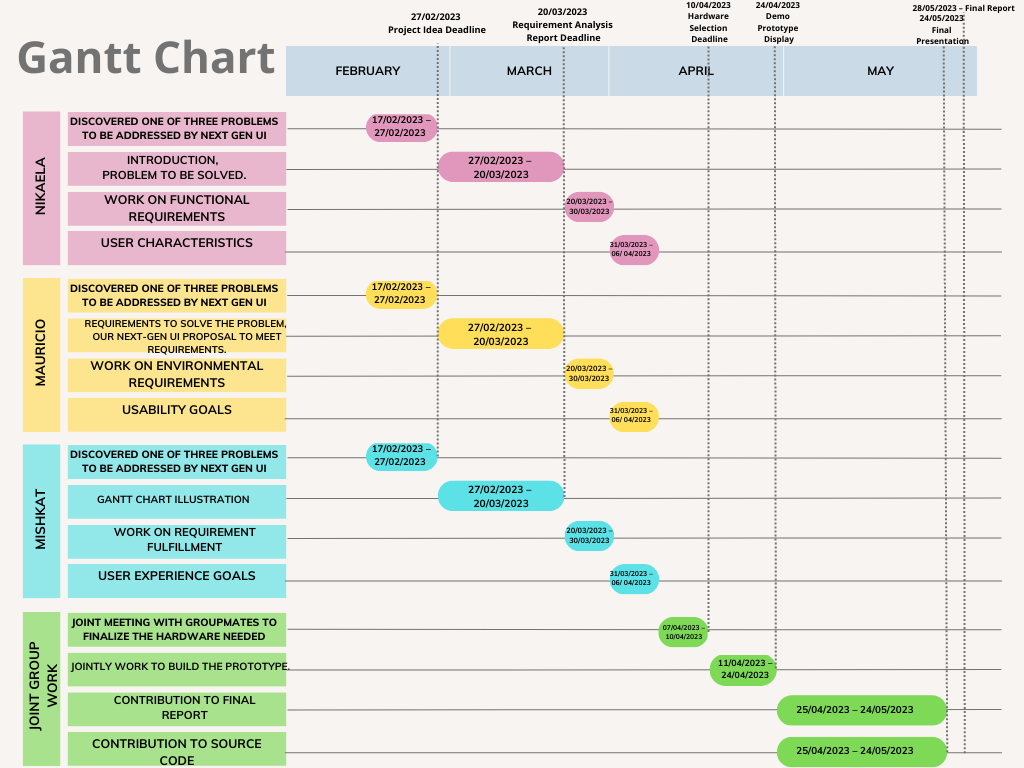
\includegraphics[width=\linewidth]{GanttChart.png}
\caption{Gantt Chart}
\label{Query results for 6th - 10th execution}
\end{figure}

\bibliographystyle{ieeetr}
\bibliography{mybib}
\end{document}
